% Copyright (c) 2026 Ali-Eimaan.
% SPDX-License-Identifier: BSD-3-Clause
%
% Authority for the equations implemented in
%   uav_mpc/src/quadrotor_dynamics.cpp   and   codegen/quadrotor_model.py.
% If the code and this file disagree, this file is wrong until proven otherwise — but they
% must not disagree in a commit.

\documentclass[11pt]{article}
\usepackage{amsmath,amssymb,amsthm,bm,geometry,hyperref,cleveref,booktabs,siunitx}
\usepackage{tikz}
\geometry{margin=1in}

\newcommand{\R}{\mathbb{R}}
\newcommand{\SO}{\mathrm{SO}(3)}
\newcommand{\SE}{\mathrm{SE}(3)}
\newcommand{\skewm}[1]{\left[#1\right]_\times}
\newcommand{\quatmul}{\otimes}
\DeclareMathOperator{\diag}{diag}

\title{Twelve-State Quadrotor Dynamics on $\SE$}
\author{Ali-Eimaan}
\date{}

\begin{document}
\maketitle

\begin{abstract}
This document derives the rigid-body quadrotor model used by the nonlinear MPC of this
repository, from Newton--Euler mechanics to the exact discrete-time map implemented in
\texttt{uav\_mpc/src/quadrotor\_dynamics.cpp} and its symbolic twin
\texttt{codegen/quadrotor\_model.py}. The model is twelve states in either of two attitude
representations: a Hamilton quaternion $(w,x,y,z)$ making thirteen states, and a ZYX Euler
angle triple making twelve. We state every assumption explicitly, derive the control
allocation map, linearise about hover to justify the discretisation and horizon choices, and
close with the geometric tracking controller used as the comparison baseline. All equations
are cross-referenced to the implementing code.
\end{abstract}

\tableofcontents

\section{Frames and notation}

\begin{itemize}
  \item World frame $\mathcal{W}$: east--north--up (ENU), right-handed. Gravity acts along
        $-\bm e_3^W$, $\bm g = (0, 0, -g)$.
  \item Body frame $\mathcal{B}$: front--left--up (FLU), right-handed, fixed to the vehicle.
  \item Rotation matrix $R \in \SO$ maps body vectors to world vectors:
        $\bm v^W = R \, \bm v^B$. Columns of $R$ are the body axes expressed in the world
        frame: $R = [\bm x_B \ \bm y_B \ \bm z_B]$.
  \item Quaternions are Hamilton, ordered $(w, x, y, z)$, with the multiplication
        convention used in \texttt{quatMultiply()} (body-to-world composition: rotating by
        $q_1$ then $q_2$ is $q_2 \quatmul q_1$).
  \item The hat map $\skewm{\bm\omega}$ is the skew-symmetric matrix such that
        $\skewm{\bm\omega} \bm v = \bm\omega \times \bm v$; the vee map is its inverse.
\end{itemize}

PX4 uses NED/FRD; the two fixed 180$^\circ$ rotations are applied only at the message
boundary in \texttt{nmpc\_node.cpp} (\texttt{enuToNed}, \texttt{quatEnuFluToNedFrd}), never
inside the dynamics. State the conventions once and loudly: half of all quadrotor bugs are a
convention mismatch.

\begin{table}[h]
\centering
\caption{Symbol table. All quantities are SI; quaternion components are dimensionless.}
\label{tab:symbols}
\begin{tabular}{@{}llll@{}}
\toprule
Symbol & Meaning & Units & Source \\
\midrule
$\bm p$ & position in $\mathcal{W}$ & m & $x_{0:3}$ \\
$\bm v$ & velocity in $\mathcal{W}$ & m/s & $x_{3:6}$ \\
$q = (w,\bm q_v)$ & attitude quaternion, $\mathcal{B}\to\mathcal{W}$ & --- & $x_{6:10}$ \\
$\bm\omega$ & body angular rate & rad/s & $x_{10:13}$ \\
$u_i$ & thrust of rotor $i$, $i=1..4$ & N & $u$ \\
$m$ & vehicle mass & kg & \texttt{params\_..mass} \\
$J$ & inertia tensor (body) & kg\,m$^2$ & \texttt{inertia} \\
$g$ & gravitational acceleration & m/s$^2$ & 9.80665 \\
$d$ & rotor lever arm in the $xy$ plane & m & $\texttt{arm\_length}/\sqrt2$ \\
$k_T$ & thrust coefficient & N/(rad/s)$^2$ & \texttt{thrust\_coeff} \\
$k_Q$ & torque coefficient & N\,m/(rad/s)$^2$ & \texttt{torque\_coeff} \\
$D$ & linear drag coefficient (body) & N\,s/m & \texttt{drag\_coeff} \\
$\tau$ & rotor time constant & s & \texttt{rotor\_time\_constant} \\
\bottomrule
\end{tabular}
\end{table}

\section{Assumptions}
\label{sec:assumptions}

\begin{enumerate}
  \item \textbf{Rigid body.} No bending; the airframe deforms negligibly under load.
  \item \textbf{Symmetric mass distribution.} $J$ is diagonal in the body frame. This fails
        for asymmetric payloads; the code accepts a full symmetric $J$ (and validates
        positive definiteness), so this is an assumption about the nominal frames, not a
        code restriction.
  \item \textbf{Rotors as pure force+torque generators.} Rotor $i$ produces thrust
        $T_i = k_T \omega_i^2$ along $+\bm z_B$ and drag torque
        $Q_i = k_Q \omega_i^2$ about $-\bm z_B$. The controller commands thrust directly
        through the allocation map; the first-order motor lag
        ($\tau_r = 12.5$ ms on the X500) is below the 100 Hz control rate and is not part of
        the model.
  \item \textbf{Linear rotor drag.} Aerodynamic force $\bm F_d = -D \bm v^B$ in the body
        frame, $D = \diag(d_x, d_y, d_z)$. This is the dominant unmodelled-in-SE(3) effect
        at the 3 m/5 s figure-8 speed; the coefficient is identified in
        \texttt{docs/TUNING\_GUIDE.md} \S5.
  \item \textbf{No ground effect, no blade flapping, flat non-rotating Earth.}
\end{enumerate}

Which assumptions does the aggressive figure-8 (3 m amplitude, 5 s period, ~5.3 m/s peak
speed, $45.8^\circ$ peak bank) actually stress? The drag term (assumption 4): at peak speed
the drag force per axis is $D_x v_x \approx 0.1 \times 3.77 \approx 0.38$ N against a
per-rotor hover thrust of 4.9 N — a few percent, but it accumulates as a systematic tracking
lag on the fast segments. Assumptions 1--3 are comfortable at this scale; 5 is validated by
the altitude margin in the SITL figure-8.

\section{Translational dynamics}

Newton's second law in the world frame. The body-frame drag is rotated into the world frame
with $R D R^{\mathsf T}$:
\begin{equation}
  \ddot{\bm p} = \frac{1}{m} R \left( \bm F_b - D R^{\mathsf T} \dot{\bm p} \right)
  + \bm g, \qquad \bm F_b = \begin{pmatrix} 0 \\ 0 \\ \sum_i u_i \end{pmatrix},
  \label{eq:trans}
\end{equation}
implemented at \texttt{quadrotor\_dynamics.cpp} lines 227--233. The drag is applied in the
body frame: the rotors create an induced flow along $-\bm z_B$, so the drag opposes the
body-relative velocity, which is the physically meaningful quantity (Faessler et al.\ 2017).

\section{Rotational dynamics}

Euler's equation in the body frame, with $\bm\tau$ the body torque from the allocation map:
\begin{equation}
  J \dot{\bm\omega} + \bm\omega \times J \bm\omega = \bm\tau
  \qquad\Longleftrightarrow\qquad
  \dot{\bm\omega} = J^{-1} \left( \bm\tau - \bm\omega \times J \bm\omega \right).
  \label{eq:rot}
\end{equation}
Implemented at \texttt{quadrotor\_dynamics.cpp} lines 259--262. The gyroscopic term
$\bm\omega \times J \bm\omega$ is small at the body rates of the figure-8 ($\lesssim 3$ rad/s)
but is retained for correctness at the 6 rad/s rate bound.

\section{Attitude kinematics}

\subsection{Quaternion}

The quaternion kinematics are the Hamilton form of $\dot R = R \skewm{\bm\omega}$:
\begin{equation}
  \dot q = \frac12 \, q \quatmul \begin{pmatrix} 0 \\ \bm\omega \end{pmatrix}.
  \label{eq:quatkin}
\end{equation}
Written as a matrix product, with $\bm q_v = (q_x, q_y, q_z)$:
\begin{equation}
  \dot q = \frac12 \begin{bmatrix}
    -q_x & -q_y & -q_z \\
    q_w & -q_z & q_y \\
    q_z & q_w & -q_x \\
    -q_y & q_x & q_w
  \end{bmatrix} \bm\omega
  = \frac12 \Omega(\bm\omega) q,
  \label{eq:quatkinmat}
\end{equation}
which is the form used in the Jacobian at \texttt{quadrotor\_dynamics.cpp} lines 340--348.
The exact flow of \eqref{eq:quatkin} preserves $\|q\|$: differentiating $\|q\|^2$ gives
$q^{\mathsf T}\dot q = \frac12 q^{\mathsf T}\Omega(\bm\omega) q = 0$ because $\Omega$ is
skew-symmetric in the $(w, \bm q_v)$ split. The RK4 discretisation does not preserve the norm
exactly, hence the renormalisation after each \texttt{step()} call
(\texttt{quadrotor\_dynamics.cpp} lines 272--276). The drift per step is $O(dt^4)$ — at
$dt = 50$ ms and rates below 6 rad/s it is below $10^{-6}$ and the renormalisation is exact.

\subsection{ZYX Euler angles}

The alternative representation uses $\bm\Theta = (\phi, \theta, \psi)$ (roll, pitch, yaw)
with $R = R_z(\psi) R_y(\theta) R_x(\phi)$:
\begin{equation}
  \dot{\bm\Theta} = T(\bm\Theta) \bm\omega, \qquad
  T = \begin{bmatrix}
    1 & \sin\phi\tan\theta & \cos\phi\tan\theta \\
    0 & \cos\phi & -\sin\phi \\
    0 & \sin\phi/\cos\theta & \cos\phi/\cos\theta
  \end{bmatrix},
  \label{eq:eulerT}
\end{equation}
singular at $|\theta| = \pi/2$ ($\det T = 1/\cos\theta$), implemented at
\texttt{quadrotor\_dynamics.cpp} lines 245--253. The quaternion representation is the default
(\texttt{attitude\_rep: quaternion}): it is singularity-free and the nonlinear least-squares
cost uses the quaternion error directly (\texttt{derivations/nmpc\_formulation.tex}
\S\ref{sec:cost}).

\section{Control allocation}
\label{sec:allocation}

The quad-X mixer. Motor numbering follows PX4's convention, which is \emph{not} the intuitive
clockwise order:
\begin{center}
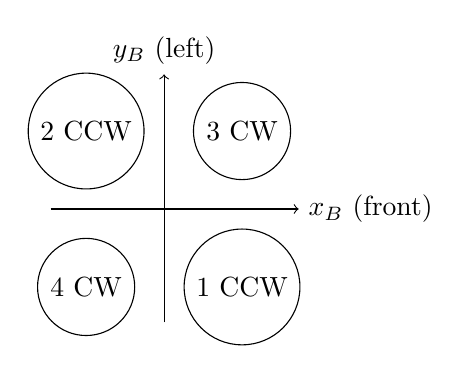
\begin{tikzpicture}[scale=0.9]
  \draw[->] (-1.6,0) -- (1.9,0) node[right] {$x_B$ (front)};
  \draw[->] (0,-1.6) -- (0,1.9) node[above] {$y_B$ (left)};
  \node at (1.1,1.1) [draw,circle] {3 CW};
  \node at (1.1,-1.1) [draw,circle] {1 CCW};
  \node at (-1.1,1.1) [draw,circle] {2 CCW};
  \node at (-1.1,-1.1) [draw,circle] {4 CW};
\end{tikzpicture}
\end{center}
\quad rotors 1 (front-right) and 2 (rear-left) spin counterclockwise; 3 (front-left) and 4
(rear-right) spin clockwise. With $d = \texttt{arm\_length}/\sqrt2$ and
$c = k_Q/k_T$, the wrench map is
\begin{equation}
  \underbrace{\begin{pmatrix} T \\ \tau_x \\ \tau_y \\ \tau_z \end{pmatrix}}_{\bm w}
  = \underbrace{\begin{bmatrix}
      1 & 1 & 1 & 1 \\
    -d & d & d & -d \\
    -d & d & -d & d \\
    -c & -c & c & c
  \end{bmatrix}}_{A}
  \underbrace{\begin{pmatrix} u_1 \\ u_2 \\ u_3 \\ u_4 \end{pmatrix}}_{\bm u},
  \label{eq:alloc}
\end{equation}
implemented at \texttt{quadrotor\_dynamics.cpp} lines 195--202. The map is invertible with
$\det A = 16\, c d^2 \neq 0$; the inverse is computed analytically at build time. The
clamped inverse used by \texttt{allocateInverse} projects the raw solution onto the box
$[u_{\min}, u_{\max}]^4$ and reports whether clamping occurred. The 3 m/5 s figure-8 on the
X500 needs peak per-rotor thrust 7.03 N against a 8.55 N limit (\S\ref{sec:lin} and
\texttt{derivations/differential\_flatness.tex} \S\ref{sec:feas}).

\section{Full state-space model}

Assembling \eqref{eq:trans}, \eqref{eq:rot}, \eqref{eq:quatkin} with state
$\bm x = [\bm p; \bm v; q; \bm\omega] \in \R^{13}$ (or $[\bm p; \bm v; \bm\Theta;
\bm\omega] \in \R^{12}$ for the Euler variant) and input $\bm u \in \R^4$:
\begin{equation}
  f(\bm x, \bm u) =
  \begin{pmatrix}
    \bm v \\
    \frac1m R \left( \bm F_b - D R^{\mathsf T} \bm v \right) + \bm g \\
    \frac12 q \quatmul \begin{pmatrix}0\\ \bm\omega\end{pmatrix} \\
    J^{-1} \left( A_{2:4,:} \bm u - \bm\omega \times J \bm\omega \right)
  \end{pmatrix}.
  \label{eq:full}
\end{equation}
Implemented in \texttt{QuadrotorDynamics::f} (\texttt{quadrotor\_dynamics.cpp} lines
212--266) and symbolically in \texttt{codegen/quadrotor\_model.py}
(\texttt{quadrotor\_model.py} lines 220--240). The symbolic model adds the online parameter
vector $\bm p = [\bm v_{\mathrm{wind}}; m_{\mathrm{scale}}; q_{\mathrm{ref}}]$
($\bm v_{\mathrm{wind}}$ in the world frame) and the wind enters through the drag term:
\begin{equation}
  \ddot{\bm p} = \frac1m R \left( \bm F_b - D R^{\mathsf T} (\bm v - \bm v_{\mathrm{wind}})
  \right) + \bm g,
\end{equation}
i.e.\ the drag opposes the body-relative velocity including wind. The quaternion error
$q_{\mathrm{ref}}^{-1} \quatmul q$ is a function of the parameter $q_{\mathrm{ref}}$ and the
state, which is why the reference attitude lives in $\bm p$ rather than in the acados
\texttt{yref} mechanism (see \texttt{nmpc\_formulation.tex} \S\ref{sec:cost}).

\section{Linearisation about hover}
\label{sec:lin}

At hover trim $\bar{\bm x}$: $\bm v = 0$, $q = (1,0,0,0)$, $\bm\omega = 0$,
$R = I$, $\bar u_i = mg/4 = 4.903$ N. Linearising \eqref{eq:full} gives the block-triangular
structure
\begin{equation}
  \delta \dot{\bm x} =
  \underbrace{\begin{bmatrix}
    0 & I & 0 & 0 \\
    0 & -\frac1m D & -\bm g^\wedge & 0 \\
    0 & 0 & 0 & \frac12 \begin{bmatrix} 0\\ I \end{bmatrix}_{\!4\times3}\\
    0 & 0 & 0 & 0
  \end{bmatrix}}_{A}
  \delta \bm x
  + \underbrace{\begin{bmatrix}
    0 \\ \frac1m \bm e_3 \bm 1_4^{\mathsf T} \\ 0 \\ J^{-1} A_{2:4,:}
  \end{bmatrix}}_{B}
  \delta \bm u,
  \label{eq:lin}
\end{equation}
with $(-\bm g^\wedge)_{ij} = -\varepsilon_{ij3}g$ the tilt--force coupling. The pair $(A,B)$
is controllable on the attitude block (the attitude dynamics are a chain of integrators
driven by the rate input), and the full system is controllable given the coupling through
$R \bm F_b$; this is checked numerically in \texttt{test\_dynamics.cpp}.

The natural time scales that justify the discretisation:
\begin{itemize}
  \item \emph{Attitude (tilt) mode:} the pendulum-like mode
        $\omega_\mathrm{tilt} \approx \sqrt{mg d / (J_{xx} + m d^2)}$. For the X500,
        $J_{xx} = 0.02166$ kg\,m$^2$, $d = 0.177$ m, giving
        $\omega_\mathrm{tilt} \approx \sqrt{mg d / J_{xx}} \approx 12.6$ rad/s —
        period $\approx 0.5$ s. With $dt = 50$ ms there are $\sim 10$ samples per tilt
        period.
  \item \emph{Body-rate mode:} driven directly by the torque input; the fastest relevant
        closed-loop bandwidth is set by the rate bound $\pm 6$ rad/s and the 100 Hz loop.
  \item \emph{Position mode:} double integrator; the slowest, so it dictates the horizon
        $T_f = 1$ s: a 1 s horizon spans $\sim 2$ tilt periods and lets the MPC see the
        consequences of a commanded tilt well before the position error accumulates.
\end{itemize}
The 50 ms/1 s choice is therefore not a guess: it resolves the fastest mode the controller
must influence with $\sim$10 samples per period, while covering the slow mode far enough to
plan. The ERK4 discretisation has local truncation error $O(dt^5)$; see
\texttt{nmpc\_formulation.tex} \S\ref{sec:disc} for the accuracy comparison.

\section{Baseline: geometric tracking control}

The comparison baseline is the Lee--Leok--McClamroch geometric controller (2010). In this
notation, with desired attitude $R_d$ and desired body rates $\bm\omega_d$,
\begin{equation}
  \bm\tau = J \left( \dot{\bm\omega}_d - \bm\omega \times \bm\omega_d \right) - \bm\omega
  \times J \bm\omega - k_R e_R - k_\omega e_\omega,
  \label{eq:geom}
\end{equation}
with the rotation error
\begin{equation}
  e_R = \frac12 \left( R_d^{\mathsf T} R - R^{\mathsf T} R_d \right)^\vee,
  \qquad e_\omega = \bm\omega - R^{\mathsf T} R_d \bm\omega_d,
\end{equation}
and the thrust $T = (m \bm a_d + m g \bm e_3) \cdot (R \bm e_3)$ from the position
controller. We cite the theorem (almost global asymptotic stability under their gain
conditions) without restating its proof; this controller is used only as the README
comparison baseline and is not part of the MPC loop.

\bibliographystyle{plain}
\bibliography{refs}

\end{document}
